%----------------------------------------------------------
\subsection{Modelo del sistema} \label{subsec:system_model}
El sistema consiste en un quadrotor portando una c\'amara. Las coordenadas de los puntos del espacio respecto a los ejes del la c\'amara son:

\begin{equation}
\left. \overrightarrow{P_{obj}} = \overrightarrow{C} + \bar{\bar{R}}^{T}*\overrightarrow{P_{c}} \right|_c
\end{equation}

\begin{equation} \label{eq:system_equation}
P_{obj} = 
	\left.
	\begin{pmatrix}
	x \\
	y \\
	z \\
	\end{pmatrix}
=
	\begin{pmatrix}
	c_x \\
	c_y \\
	c_z \\
	\end{pmatrix}
+
	\begin{pmatrix}
	r_{11} & r_{21} & r_{31} \\
	r_{12} & r_{22} & r_{32} \\
	r_{13} & r_{23} & r_{33} \\
	\end{pmatrix}
*
	\begin{pmatrix}
	x_c \\
	y_c \\
	z_c \\
	\end{pmatrix}
	\right|_c
\end{equation}


%----------------------------------------------------------
\subsection{Camera Model}
	El modelo de la c\'amara \cite{camera_models}  y sus ecuaciones fueron descritas en la secci\'on del algoritmo de matching.
	
	\begin{figure}[ph]
		\centering
		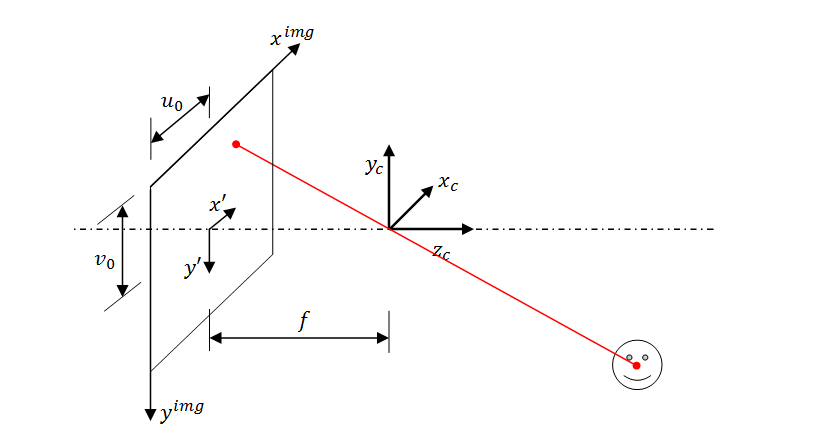
\includegraphics[width=0.7\linewidth]{../Images/c2/pinhole_model}
		\caption{}
		\label{fig:pinhole_model}
	\end{figure}

	
%----------------------------------------------------------
\subsection{Extended Kalman Filter}

El filtro de Kalman es un algoritmo iterativo de estimaci\'on de estados de sistemas din\'amicos. Este suele ser aplicado cuando se necesita saber el estado de un sistema con m\'as mediciones que grados de libertad del sistema y para la atenuaci\'on de ruido blanco en las estimaciones. En este caso usamos una aproximaci\'on lineal del sistema con una variante llamada Filtro de Kalman Extendido \cite{GabrielTerejanu_EKF} (o EKF).

Sea el sistema a estudiar:

\begin{gather}
x_k = f(x_{k-1}) + w_{k-1} \\
z_k = h(x_k) + v_k
\end{gather}

Cada paso del EKF esta formado de dos iteraciones llamadas "Predictor" y "corrector"

\begin{itemize}
   \item Predictor Step
		\begin{gather}
			x_k^{f} \approx f(x_{k-1}^{a}) \\
			P_k^{f} = J_f(x_{k-1}^{a}) P_{k-1} J_f^{T}(x_{k-1}^{a}) + Q_{k-1}
		\end{gather}

	\item Corrector Step
		\begin{gather}
			P_k = (I - K_k J_h(x_k^{f}))P_k^{f} \\
			K_k = P_k^{f} J^{T}_h(x_k^{f}) (J_h(x_k^{f}) P_k^{f} J_h^{T}(x_k ^{f}) + R_k)^{-1} \\
			x_k^{a} \approx x_k^{f} + K_k (z_k - h(x_k^{f}))
		\end{gather}
\end{itemize}